
\section{Formulación de control óptimo para el problema SHE}

En esta sección presentaremos la formulación de un problema de control para el problema SHE de dos niveles. Este se puede formalizar de la siguiente manera:

\begin{problem}[OCP para SHE de dos niveles]\label{OCP1}
    Dados dos conjuntos de números impares $\mathcal{E}_a$ and $\mathcal{E}_b$ con cardinalidades $|\mathcal{E}_a| = N_a$ y  $|\mathcal{E}_b| = N_b$ respectivamente , dados los vectores objetivos $\bm{a}_T  \in \mathbb{R}^{N_a}$ y $\bm{b}_T  \in \mathbb{R}^{N_b}$, buscamos la función  $f(\tau ) \ | \ \tau \in (0,\pi)$ que minimiza el siguiente funcional de coste:
        \begin{gather}
        J[f(\tau)] = \Bigg[ || \bm{a}_T - \bm{\alpha}(T)||^2 + || \bm{b}_T - \bm{\beta}(T)||^2 
        + \epsilon \int_0^{\pi} \mathcal{L}(f) d\tau \Bigg] 
    \end{gather}

    donde  $\bm{\alpha}(\tau) \in \mathbb{R}^{N_a} \times [0,\pi]$, $\bm{\beta}(\tau) \in \mathbb{R}^{N_b}  \times [0,\pi]$,  $||.||$ es la norma euclidea y $\epsilon$ es un parámetro pequeño que penaliza el funcional de coste con el término $\mathcal{L}(f):\mathbb{R} \rightarrow \mathbb{R}$. 
    \newline

    De esta forma podemos escribir el siguiente problema de control óptimo:
    \begin{gather}
        \min_{|f(\tau) |<1} J[f(\tau)] \\
        \notag \text{suject to: } \\
        \notag \forall i \in \mathcal{E}_a\ \ 
        \begin{cases}
            \dot{\alpha}_i(\tau) = (2/\pi) \cos(i\tau) f(\tau) & \tau \in [0,\pi]\label{dyn}\\
            \alpha_i(0) = 0
        \end{cases} \\
        \notag \forall j \in \mathcal{E}_b\ \ 
        \begin{cases}
            \dot{\beta}_j(\tau) = (2/\pi) \sin(j\tau) f(\tau) & \tau \in [0,\pi]\label{dyn}\\
            \beta_j(0) = 0
        \end{cases} \\
    \end{gather}
\end{problem}

En el problema de SHE de dos niveles se busca una función $\{f(\tau) \ |  \tau \in [0,\pi] \}$  que solo pueda tomar los valores $\{-1,1\}$, sin embargo el problema (\ref{OCP1}) definido para un término de penelización $\mathcal{L}(f)$ arbitrario puede tomar valores en todo el intervalo $[-1,1]$. 
%
En teoría de control los controles que toma solo los valores extremos del intervalo son conocidos como controles \emph{bang-bang}, estos se pueden obtener en condiciones muy concretas, como el tiempo mínimo de control. 

A continuación estudiaremos las condiciones de optimilidad del problema con el fin de encontrar condiciones en el término $\mathcal{L}(f)$ que nos de el comportamiento \emph{bang-bang} en el control óptimo. Entonces siguiendo el principio de mínimo de Pontryagin, escribimos el Hamiltoniano del problema:

\begin{gather}\label{hamil}
    H(f,\bm{p}^\alpha(\tau),\bm{p}^\beta(\tau),\tau) = \epsilon \mathcal{L}(f) + 
    G(\bm{p}^\alpha(\tau),\bm{p}^\beta(\tau),\tau) f(\tau)
\end{gather}

Donde  hemos llamado $G(\bm{p}^\alpha,\bm{p}^\beta,\tau)$ a:
    \begin{gather}
        G(\bm{p}^\alpha,\bm{p}^\beta,\tau) = \frac{2}{\pi} \Bigg[ 
            \sum_{i \in \mathcal{E}_a} p^\alpha_i \cos(i\tau)+ 
            \sum_{j \in \mathcal{E}_b} p^\beta_j \sin(j\tau) 
        \Bigg]
    \end{gather}

y además donde $\bm{p}^\alpha(\tau) \in \mathbb{R}^{N_a} \times [0,\pi]$ y $\bm{p}^\beta(\tau) \in \mathbb{R}^{N_b}  \times [0,\pi]$ son los estados adjuntos correspondientes a los estados $\bm{\alpha}$ y $\bm{\beta}$ respectivamente. 
\newline 

Utilizando la siguiente condición de optimalidad:

\begin{gather}\label{minH}
    H(\tau,\bm{p}_*^\alpha,\bm{p}^\beta_*,f_*) \leq
    H(\tau,\bm{p}_*^\alpha,\bm{p}^\beta_*,f)
\end{gather}

podemos obtener la forma del control óptimo cuando los co-estados óptimos $\bm{p}_*^\alpha$ y $\bm{p}_*^\beta$ además de la variable temporal $\tau$ están fijas. 
%
Entonces el problema se reduce la minimización de una función $H^*(f) = H(\tau,\bm{p}_*^\alpha,\bm{p}^\beta_*,f)$ en una variable $f$ dentro de un intervalo $[-1,1]$.
%
Dado que necesitamos que el control óptimo $f^*$ sea \emph{bang-bang}, debemos diseñar  $H^*(f)$ de manera que su mímino esté en los extremos del intervalo.
%
En el caso de una variable (este caso) solo podemos conseguir este comportamiento si no existe ningún mínimo dentro del intervalo. Una manera de asegurar este comportamiento es tomando la función $H^*(f)$ concava, mediante la elección el término $\mathcal{L}(f)$. Eso se debe a que la concavidad de el término $\mathcal{L}(f)$ determina la concavidad del Hamiltoniano $H^*(f)$ gracias a que la derivada segunda de $H^*(f)$ es proporcional al la derivada segunda del término de penalización, es decir:
\begin{gather}
    \frac{d^2{H^*}^2}{df^2} = \epsilon \frac{d^2\mathcal{L}(f)}{df^2} 
\end{gather}

Así que siempre que elijamos un término de penalización tal que:

\begin{gather}
    \frac{d^2L[f]}{df^2} \leq 0 
\end{gather}

obtendremos un función $H^*(f)$ cóncava dentro de un intervalo convexo dando lugar a un control óptimo $f^*$  \emph{bang-bang}. Podemos ver una ilustración de este comportamiento en la figura (\ref{bang-bang})
\newline

\begin{figure}[!ht]
    \centering
    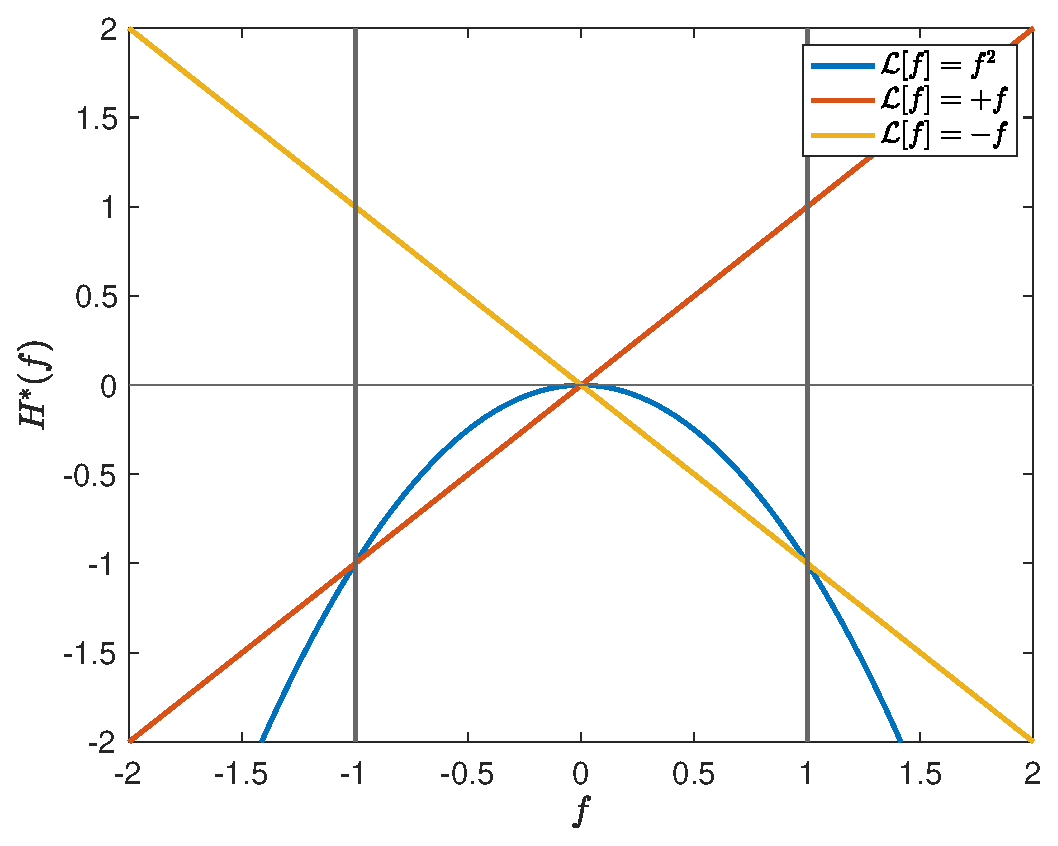
\includegraphics[scale=0.5]{img/bang-bang.eps}
    \caption{Ilustración sobre el comportamiento de la función $H^*(f)$ para distintos términos de penalización $\mathcal{L}(f)$. El problema de minimización de $H^*(f)$ con respecto a $f$ para las distintas curvas presentadas en la figura siempre tiene minimos en los extremos del intervalo $[-1,1]$ de manera que el control óptimo en los tres casos, será \emph{bang-bang}.}
    \label{bang-bang}
\end{figure}


\subsection{OC SHE de dos niveles con simetría de cuarto de onda} 

Consideraremos un caso concreto del problema presentado en la sección anterior. Este es problema de SHE con simetría de cuarto de onda, es decir consideramos que la función $f(\tau)$ cumple la siguiente expresión:
\begin{gather}
    f(\tau + \pi/2)   = f(\tau)    \ | \ \tau \in (0,\pi/2)
\end{gather}

Esta expresión nos permite simplificar la expresión para los coeficientes de Fourier (\ref{an}) and (\ref{bn}) de la siguiente manera:
\begin{align}
    a_i = & \  0 \ \ | \  \ \forall i \in \mathbb{Z} \\
    b_j = &  \frac{4}{\pi} \int_0^{\pi/2} f(\tau ) \sin(j\tau)d\tau \ | \ \forall j \ odd
\end{align}

Entonces  $f(\tau) \ | \ \tau \in (0,\pi/2)$ puede ser escrita como:
\begin{gather}
    f(\tau ) = \sum_{j \ odd}^\infty  b_j \sin(j \tau) \\
    b_j = \frac{4}{\pi}\int_0^{\pi/2} f(\tau ) \sin(j\tau)d\tau \ \ | \ \ j \ odd \label{bn_odd}
\end{gather}

En este contexto podemos definir el problema de control de manera análoga que en la subsección anterior:
\begin{problem}\label{OCP_bn}
    Dado un conjunto de número impares $\mathcal{E}_b$ con cardinalidad $|\mathcal{E}_b| = N_b$ y dado un vector objetivo $\bm{b}_T  \in \mathbb{R}^{N_b}$, buscamos la función $f(\tau ) \ | \ \tau \in (0,\pi/2)$ tal que  $f(\tau)$ minimize el siguiente funcional de coste:

        \begin{gather}
        J[f(\tau)] = \Bigg[ || \bm{b}_T - \bm{\beta}(T)||^2 + \epsilon \int_0^{\pi/2} \mathcal{L}(f(\tau)) d\tau \Bigg] 
    \end{gather}

    donde $ \bm{\beta}(\tau) \in \mathbb{R}^{N_b} \times [0,\pi/2] $,  $||.||$ es la norma euclidea y $\epsilon$ es un parámetro de penalización para el término $\mathcal{L}(f)$
    \newline

    Entonces el problema de control se puede escribir como:
    \begin{gather}
        \min_{|f(\tau) |<1} J[f(\tau)] \\
        \notag \text{suject to: } \\
        \notag \forall j \in \mathcal{E}_b \
        \begin{cases}
            \dot{\beta_j}(\tau) = (4/\pi) \sin(j\tau) f(\tau) & \tau \in [0,\pi/2]\label{dyn}\\
            \beta_j(0) = 0
        \end{cases} 
    \end{gather}
\end{problem}

En este caso el problema de control tiene el siguiente Hamiltoniano:
\begin{gather}
    H(f,\bm{p}_\beta,\tau) = \epsilon  \mathcal{L}(f)+ 
    \frac{4f}{\pi} \Bigg[ 
        \sum_{j \in \mathcal{E}_b} p^\beta_j \sin(j\tau) 
    \Bigg]
\end{gather}

Podemos ver que el Hamiltoniano tiene la misma estructura que en la subsección anterior, por lo que de la misma forma la elección de un término de penalización $\mathcal{L}(f)$ concavo nos produce un Hamiltoniano $H^*(f)$ cóncavo y por tanto un control óptimo $f^*$ \emph{bang-bang}.
